%===============================
%------------------------------
\section{Mathematical Prerequisite}
%------------------------------
%===============================


%---------------------------------------------
\subsection{Transition from wave mechanics}
%---------------------------------------------



The stationary states from a complete, orthonormal set
\begin{empheq}[box=\fbox]{align}
	\int dx\, \varphi_n^* (x) \varphi_m(x) &= \delta_{nm}
	\mnf{Orthonormality} \label{eq:orthogonality-function-space}  \\
\sum_{n} \varphi_n^*(x) \varphi_n(x') &= \delta(x-x')
\mnf{Completeness \mbox{(Closure relation)}} \label{eq:completeness-function-space}
\end{empheq}
The Dirac delta ``function" is a generalized function, also known as a distribution, and only has meaning inside an integral.
\begin{align}
	\int dx'\, f(x') \delta(x-x') = f(x)
\end{align}
Think of the delta function as a linear map from $\hilb$ to $\C$.

Given a function $\psi(x)$. Suppose that we can write
\begin{align}\label{eq:expansion-function-space}
	\psi(x) &= \sum_n c_n \varphi_n(x).
\end{align}
Orthogonality implies that
\begin{align}
	\int dx\, \varphi_n^*(x)\psi(x) 
	&= \sum_m c_m \int dx\, \varphi^*_n(x)\varphi_m(x)  \\
	&= \sum_m c_m \delta_{nm} = c_n.
\end{align}
In other words, we have an identity
\begin{align}
	\boxed{c_n = \int dx\, \varphi_n^*(x)\psi(x) }\,.
\end{align}
Equipped with the orthonormality relation, we can show that the closure relation is equivalent to the spanning property.\mn{Of course, a set that is not orthonormal (nor orthogonal) can also span the space, in which case the closure relation is generalized to the \href{https://en.wikipedia.org/wiki/Frame_(linear_algebra)}{\emph{frame condition}}.}
\begin{lemma}\label{}
	An orthonormal set $\{\varphi_n(x)\}_n$ spans the space of function if and only if it satisfies the closure relation \eqref{eq:completeness-function-space}.
\end{lemma}
\begin{proof}
	``$\impliedby$" direction
	
	Suppose that the closure relation is true. For an arbitrary $\psi(x)$, compute $\psi(x) = \sum_n c_n \varphi_n(x)$. We want to show that $\sum_nc_n\varphi_n(x)$ is nothing but $\psi(x)$.
	\begin{align}
		\sum_nc_n\varphi_n(x) &= \int dx'\, \psi(x') \sum_n \varphi_n^*(x') \varphi_n(x) \\
		&= \int dx'\, \psi(x')\delta(x-x') = \psi(x)
	\end{align}
	as desired.
	
	``$\implies$" direction
	
	Suppose that the expansion \eqref{eq:expansion-function-space} is valid for an arbitrary function,
	\begin{align}
		\psi(x) &=  \int dx'\, \psi(x') \sum_n \varphi_n^*(x') \varphi_n(x),  
	\end{align}
	then it must be that the sum acts like a Dirac delta function, which completes the proof.
\end{proof}

In quantum theory, $\abs{c_n}^2$ has the meaning of the probability to find the system in the state $\varphi_n(x)$. It is straightforward to verify that
\begin{align}
	\sum_n \abs{c_n}^2 = \int dx\, \abs{\psi(x)}^2.
\end{align}
More generally, if $\psi(x) = \sum_n c_n \varphi_n(x)$ and $\phi(x) = \sum_n d_n \varphi_n(x)$. Then the inner product in the function space is the same as the inner product between infinitely long vectors of sequences $\{c_n\}_n$ and $\{d_n\}_n$:
\begin{align}
	\int dx\, \phi^*(x)\psi(x) &= \sum_{nm} d_n^* c_m \int dx\, \varphi_n^*(x) \varphi_m(x) \\
	&= \sum_{nm} d_n^* c_m \delta_{nm} = \sum_n d_n^* c_n \\
	&= \mqty(d_1^*&d_2^*&\dots)\mqty(c_1\\c_2\\ \vdots)
\end{align}
Technically, these two kinds of inner product define different Hilbert spaces. One is the space $l^2$ of \emph{square-summable} sequences, 
\begin{align}
	\sum_n \abs{c_n}^2 < \infty.
\end{align}
The other is the space $L^2$ of \emph{square-integrable} functions, 
\begin{align}
	\int dx\, \abs{\psi(x)}^2 < \infty.
\end{align}

In Heisenberg's original conception of quantum theory, he rejected ascribing (continuous-valued) dynamical variables such as position and momentum to atomic orbitals on the basis that they are unobservable and that a theory that included them so far had failed to make the correct prediction \cite{jammer}. 
Heisenberg focused instead on discrete quantities $n=1,2,\dots$ that label the atomic orbitals.
In this approach, known as \emph{matrix mechanics}, there are only observables and ``quantum jumps" between different values of an observable. 
Notably, there is no notion of a quantum state\mn{So one is spared from having to physically interpret a superposition of quantum states.}, but one can think of the coefficients $\{c_n\}_n$ as a ``state". Thus, one is working in the Hilbert space $l^2$ of square-summable sequences.

Schr\"odinger came from a different vantage point entirely. He took seriously de Broglie's idea that associated to every quantum particle is a wave and asked what the wave equation for de Broglie's waves are. This led to the Schr\"odinger equation and the approach known as \emph{wave mechanics}. 
In this approach, there are only states, but no probability, at least at first.\mn{Schr\"odinger hihmself even mistakenly believed that the wave function describes a charge density of some sort.} 
It was Max Born that supplemented the probabilistic interpretation in this approach. As a result, one is working in the Hilbert space $L^2$ of square-integrable functions.

However, the two approaches were the same all along as the two Hilbert spaces are equivalent (Riesz-Fischer theorem).
From this line of thinking, John von Neumann developed a unified formulation of quantum mechanics as we know today \cite{landsman,jammer}. For us, the whole point is that $\{c_n\}_n$ and $\psi(x)$ are simply two representations of the same element  $\ket{\psi}$ of an abstract Hilbert space $\hilb$.

\begin{example}[Particle in a box]\leavevmode
	\begin{align}
		\ket{\varphi_n} \longleftrightarrow \varphi_n(x) = \sqrt{\frac{2}{L}} \cdot
		\begin{cases}
			 \sin(k_n x), & \textrm{even}\, n, \\
			 \cos(k_n x), & \textrm{odd}\, n,
		\end{cases}
	\end{align}
	where $k_n = n\pi/L$.
Note the important fact that the ket $\ket{\varphi_n}$ has no $x$-dependence.
\end{example}

\begin{example}[Spin-1/2]\leavevmode
	\begin{align}
		\ket{\psi} = \alpha\ket{\uparrow} + \beta\ket{\downarrow}
	\end{align}
\end{example}



%---------------------------------------------
\subsection{Inner product spaces}
%---------------------------------------------

The prerequisites of this section are definitions and basic properties related to vector spaces and linear operators, which can be found in Appendix \ref{sec:A01}.

%From a logical standpoint, finite and infinite-dimensional Hilbert spaces are the same. A finite-dimensional Hilbert space is a vector space equipped with an inner product.
\begin{definition}
A pairing
	\begin{align}
		V\times V &\to\C, \\
		\phi,\psi &\mapsto (\varphi,\psi)
	\end{align}
is said to be an {\bf inner product} if the following properties are satisfied.
	\begin{itemize}
		\item \emph{Linearity in the second argument}: 
		\begin{align}
			(\phi, a\psi_1 + b\psi_2) = a(\phi,\psi_1) + b(\phi,\psi_2) 
			\label{eq:inner-product-linearity}
		\end{align}
		\item \emph{Conjugate symmetry:}
		\begin{align}
			(\psi,\phi) = (\phi,\psi)^*
			\label{eq:inner-product-conjugate-symmetry} 
		\end{align}
		\item \emph{Positive-definiteness:} 
		\begin{align}
			(\psi,\psi) \ge 0 \;\textrm{with equality iff} \ket{\psi} = 0 
			\label{eq:inner-product-+ve-definite}
		\end{align}
	\end{itemize}
\end{definition}



Inner products in real vector spaces are bilinear, but inner products in complex vector spaces are  \emph{sesquilinear} they are , i.e., they are conjugate linear in the first argument. Sesquilinearity follows from \eqref{eq:inner-product-linearity} and \eqref{eq:inner-product-conjugate-symmetry}
\begin{align}
	(a\phi_1 + b\phi_2,\psi) &= (\psi,a\phi_1 + b\phi_2)^* \\
		&= a^*(\psi,\phi_1)^* + b^*(\psi,\phi_2)^* \\
		&= a^* (\phi_1,\psi) + b^*(\phi_2,\psi) 
\end{align}
Sesquilinearity is required to make $(\psi,\psi)$ non-negative. %We will see that sesquilinearity has consequence to how we define the adjoint of a linear operator, from which the whole business about the spectral theorem slides down.

\begin{example}[Weird inner product]\leavevmode
	
	The following formula defines an inner product in $\R^2$.
	\begin{align}
		(x,y) = 5x_1y_1 + x_1y_2 + x_2y_1 + 3x_2y_2.
	\end{align}
	The positive definiteness can be shown by noting that
	\begin{align}
		(x,x) = 5x_1^2 + 2x_1x_2 + 3x_2^2 = (x_1+x_2)^2 + 4x_1^2 + 2x_2^2 \ge 0,
	\end{align}
	with equality iff every term is zero.
\end{example}

%Obviously the dot product is an inner product. But is there anything else? An inner product can be equivalently given by a bilinear form (or sesquilinear in complex vector spaces).

An inner product with a fixed vector $\phi$ always can be thought as a mapping
\begin{align}
	(\phi, \_ \,): V &\to \C, \\
	\psi &\mapsto (\phi,\psi)
\end{align}
This is an example of a \emph{linear functional}, a linear map from $V$ to $\C$.
%This is a linear map from a vector space $\hilb$ to the one-dimensional vector space $\C$. Thus, it can be represented by  a 1-by-d matrix.

\begin{definition}
	The {\bf dual space} $V^*$ of $V$ is defined as the vector space of linear functionals with addition defined as\mn{Scalar multiplication in $V^*$ follows directly from the the linearity of linear functionals: $f(a\psi)=af(\psi)$.}
	\begin{align}
		(f+g)(\psi) = f(\psi) + g(\psi).
	\end{align} 
	%Furthermore, we write the action of any linear functional $f\in V^*$ on $\ket{\psi} \in V$ as
	%\begin{align}
	%	\av{f|\psi} \equiv f(\psi).
	%\end{align}
	%$\bra{f}$ is called a {\bf bra}.
	 %represented by bras $\bra{\phi}$. 
\end{definition}

\begin{lemma}
	$\dim V^* = \dim V$.
\end{lemma}
%\noindent A formal proof can be given as follows.
\begin{proof}	
	For any given basis $\{e_j\}_j$ for $V$, we can define a basis $\{f_k\}_k$ for $V^*$ by the relation $f_k(e_j) = \delta_{jk}$. If there is an element $g$ of $V^*$ that cannot be represented as a linear combination of $\{f_k\}_k$, then $g(e_j) = 0$ for every $j$, which implies that $g$ is the zero map. Therefore, $\{f_k\}_k$ spans $V^*$ and there are $\dim V$ of them.
\end{proof}
For finite dimensional vector spaces, the characterization of linear functionals are obvious in matrix form. By definition, any linear map from an $n$-dimensional vector space to $\C$ can be represented by a 1-by-$n$ matrix, 
\begin{align}
	f\left[\mqty(c_1\\c_2\\ \vdots \\ c_n)\right] = \mqty(* & * &\dots & *) \mqty(c_1\\c_2\\ \vdots \\ c_n),
\end{align}
which suggests that all linear functionals can be realized as an inner product.\mn{But note that the notion of linear functionals of the dual space does not require the notion of an inner product.} 
This is indeed true (Riez representation theorem). An inner product induces an antilinear map $\dgg$ that identifies $V$ and $V^*$,
\begin{align}
	\ket{\psi} \overset{\dagger}{\longleftrightarrow} \bra{\psi}, 
\end{align}
but the specification of the map itself will depend on the choice of the inner product. If we choose an orthonormal basis $\{\ket{e_j}\}_{j=1}^n$,
\begin{align}
	(e_j,e_k) = \delta_{jk},
\end{align} 
this map is
\begin{align}
	c_1 \ket{e_1} + \dots + c_n\ket{e_n} \overset{\dagger}{\longleftrightarrow} 
		c_1^* \bra{e_1} + \dots + c_n^*\bra{e_n}.
\end{align}
In other words, $f \in V^*$ is identified with the vector $\phi_f = \sum_j[f(e_j)]^* e_j \in V$, for suppose that $\psi = \sum_j c_j e_j$, then
\begin{align}
	(\phi_f,\psi) &= \sum_j c_j (v_f,e_j) \mnf{Linearity in the second argument} \\
	&= \sum_{jk} c_j  \{[f(e_k)]^*\}^* (e_k,e_j) = \sum_{jk} c_j  [f(e_k)] \delta_{jk} \mnf{Conjugate linearity in the first argument} \\
	&= \sum_j c_j f(e_j) = f\left[\sum_j c_j e_j\right] = f(\psi),
\end{align}
as it should be.



\begin{theorem}[\bf Cauchy-Schwarz]\leavevmode\label{thm:CS-ineq}

$$\abs{\braket{\phi}{\psi}}^2 \le \braket{\phi} \braket{\psi}$$
\end{theorem}

\begin{marginfigure}
	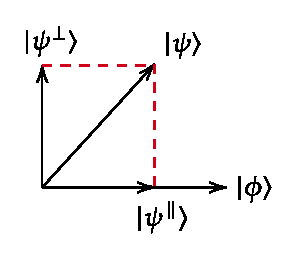
\includegraphics[scale=1]{fig/pythagorean.pdf}
	\caption{}
	\label{fig:pythagorean}
\end{marginfigure}
\begin{proof}
	Given a pair of vectors $\ket{\phi}$ and $\ket{\psi}$, one can consider the triangle formed by $\ket{\psi^{\parallel}}$, the component of $\ket{\psi}$ parallel to $\ket{\phi}$:
	\begin{align}
		\ket*{\psi^{\parallel}} = 
		\frac{\av{\phi|\psi}}{\av{\phi|\phi}}\ket{\phi}, 
	\end{align}
	and the perpendicular component $\ket{\psi^{\perp}} = \ket{\psi} - \ket*{\psi^{\parallel}}$, see Fig \ref{fig:pythagorean}.
	
	
	The Pythagorean theorem tells us that
	\begin{align}
		\braket{\psi}  &= \braket*{\psi^{\perp}} + \braket*{\psi^{\parallel}} \\
		\braket{\psi} - \frac{\abs{\braket{\phi}{\psi}}^2}{\braket{\phi}} &= \braket*{\psi^{\perp}} \ge 0
		\label{eq:pythagorean}.
	\end{align}
	from which the Cauchy-Schwarz inequality
	\begin{align}
		\abs{\av{\phi|\psi}}^2 &\le \av{\phi|\phi}\av{\psi|\psi}
	\end{align}
emerges.
	Additionally, we see from \eqref{eq:pythagorean} that the inequality is tight iff $\ket{\phi}$ and $\ket{\psi}$ are scalar multiple of each other.
\end{proof}

\begin{definition}
	The norm of $\ket{\psi}$ is $\norm{\ket{\psi}} \equiv \norm{\psi} \coloneqq \sqrt{\braket{\psi}}$.
\end{definition}
\noindent Since an inner product defines a norm, a Hilbert space is also a normed vector space.\mn{The converse is not true. Even though an inner product can be constructed from the 2-norm via the \href{https://en.wikipedia.org/wiki/Polarization_identity}{polarization identity}, (the $p$-norm is defined as $\norm{\psi}_p = \sqrt[p]{\sum \abs{c_j}^p}$), a normed space is not always an inner product space.  Take the max norm, $\norm{\psi}_{\infty} = \max_j \abs{c_j}$, for example.} By definition, a norm needs to satisfy the triangle inequality
\begin{align}
	\norm{\ket{\psi}+\ket{\phi}} \le \norm{\psi} + \norm{\phi}.
\end{align}
But for a norm induced from an inner product, the triangle inequality can be proved using the Cauchy-Schwarz inequality. Since the latter holds for any inner product, the former holds irrespective of the choice of inner product used to define the norm.
\begin{proof}
	\begin{align}
		\norm{\ket{\psi}+\ket{\phi}}^2 
		&= \norm{\psi}^2 + \norm{\phi}^2 + 2\mathrm{Re}\braket{\psi}{\phi} \\
		&\le \norm{\psi}^2 + \norm{\phi}^2 + 2\abs{\braket{\psi}{\phi}} \\
		&\le \norm{\psi}^2 + \norm{\phi}^2 + 2\norm{\psi}\cdot \norm{\phi}\mnf{Cauchy-Schwarz inequality} \\
		&= (\norm{\psi} + \norm{\phi})^2
	\end{align}
\end{proof}


The vector space in quantum theory is a \emph{separable Hilbert space}. A {\bf Hilbert space}, denoted by $\hilb$, is a vector space equipped with an inner product and some convergence properties. Separability means that there exists a countable basis for the space.\mn{Stationary states $\ket{\varphi}_n$ form a countable basis, but continuous eigenvectors such as $\ket{x}$ do not.} Additionally, since the norm of a vector has the meaning of a probability, we demand that the norm of every vector is finite. (As a consequence of the Cauchy-Schwarz inequality, this also means that every inner product is finite.) For a finite-dimensional vector space, all these issues about separability and finiteness of the norm never arises; in this case, a Hilbert space \emph{is simply an inner product space}.


\begin{mybox}
	Given the correspondence between linear functionals and the inner product, the \emph{bra-ket} $\av{v|u}$
	is often regarded as merely another notation for the inner product between two vectors in the Hilbert space.
	This interpretation is always valid in finite dimensions, but in an infinite-dimensional Hilbert space, there are linear functionals that have no corresponding vector. Take the bra $\bra{x}$, for example. Its squared norm is 
	\begin{align}
		\braket{x} = \int dx' \braket{x}{x'}\braket{x'}{x} = \int dx' \delta^2(x-x') = \delta(0) = \infty.
	\end{align}
\end{mybox}


Now we are ready to write down properties of an {\bf orthonormal basis (ONB)} in the Dirac notation. 
\begin{empheq}[box=\fbox]{align}
	\av{e_j|e_k} &= \delta_{jk}\label{eq:orthonormality} \mnf{Orthonormality} \\
\sum_j \dyad{e_j} &= \op \id \label{eq:completeness} \mnf{Completeness}
\end{empheq}
The equivalence of the spanning property and \eqref{eq:completeness} can be shown similar to the continuous case.
Suppose
\begin{align}
	\ket{\psi} = \sum_j c_j \ket{e_j}.
\end{align}
Then
\begin{align}
	\av{e_j|\psi} &= \sum_k c_k \av{e_j|e_k} \\
		&= \sum_k c_k \delta_{jk} = c_j.
\end{align}
That is, we have that
\begin{align}
	\boxed{c_j = \av{e_j|\psi}}\, .
\end{align}
Then suppose that an arbitrary vector can be expanded in such a way,
\begin{align}
	\ket{\psi} &= \sum_j c_j \ket{e_j} = \sum_j \ket{e_j}\av{e_j|\psi}. 
\end{align}
Then it must be the case that $\sum_j \dyad{e_j} = \hat \id$.




%---------------------------------------------
\subsection{Linear operators}
%---------------------------------------------

Any linear operator takes as an input a vector and outputs another vector. From this we observe that a ket-bra like $\dyad{\psi}{\phi}$ is a linear operator since
\begin{align}
	\ket{\psi}\av{\phi|\zeta} = \av{\phi|\zeta}\ket{\psi}, 
\end{align}
which is again a vector.\mn{In particular, the vector space of linear operators on $\hilb$ is $\hilb^* \otimes \hilb$.} This is the magic of the bra-ket notation. 


If an orthonormal set $\{\ket{\varphi_j}\}_j$ spans a subspace $S \subset V$, then 
\begin{align}
	\op P_S = \sum_j \dyad{e_j} 
\end{align}
is a projection operator onto the subspace $S$ and
$\op \id - \op P_S$
is the projection operator onto the orthogonal complement $S^{\perp}$. That is, the total space is the direct sum
$V = S \oplus S^{\perp}$,
and for $\ket v = \ket s + \ket p\in V$, where $s\in S$ and $p\in S^{\perp}$, we have that $\op P_S\ket v = \ket s$ and $(\op\id - \op P_S)\ket v = \ket p$.

\vspace{0.5em}
\noindent {\bf Matrix elements.}
\begin{align}
	\op T &= \hat\id \op T \hat\id = \sum_{jk} \ket{e_j} {\color{maincolor}\overbrace{\bra{e_j}\op T \ket{e_k}}^{T_{nm}}} \bra{e_k} 
\end{align}
\begin{align}
	\op T\ket{\psi} &= \sum_{jk} T_{jk} {\color{eqcolor}\overbrace{\av{e_k|\psi}}^{c_k}} = \sum_j {\color{darkmagenta}\overbrace{\left(\sum_k T_{jk}c_k \right)}^{d_j}} \ket{e_j} \\
	&\leftrightarrow \mqty(d_1 \\ d_2 \\  \vdots \\ d_n) = \mqty(T_{11}&T_{12}& \dots & & T_{1n} \\ T_{21}& T_{22} & & & \vdots \\ \vdots & & \ddots & & \\ T_{n1} & \dots & & & T_{nn})  \mqty(c_1 \\ c_2 \\ \vdots \\ c_n)
\end{align}
We see that the components transform as
\begin{align}\label{eq:transform-component}
	\boxed{d_j = \sum_k T_{jk} c_k}\,.
\end{align}
The transformation of basis vectors is in a sense ``opposite":
\begin{align}\label{eq:transform-basis}
	\boxed{\op T \ket{e_j} = \sum_k T_{kj}\ket{e_k}}.
\end{align}
The merit of the Dirac notation is that it streamlines matrix multiplications.
\begin{align}
	\op T \op S &= \sum_{jklm} T_{jl}S_{mk} \ket{e_j}\av{e_l|e_m}\bra{e_k}	
	= \sum_{jk} {\color{teal}\underbrace{\left(\sum_l T_{jl}S_{lk}\right)}_{(\op T \op S)_{nm}}}  \dyad{e_j}{e_k} 
\end{align}
For example, \eqref{eq:transform-basis} can be derived without breaking a sweat.
\begin{align}
	\op T\ket{e_j} &= \sum_{kl} T_{kl} \ket{e_k}\av{e_l|e_j} = \sum_{jk} T_{kj} \ket{e_k}
\end{align}
The same is true for \eqref{eq:transform-component}.
\begin{align}
	d_j &= \mel{e_j}{\op T}{\psi} = \sum_{klm} T_{kl} c_m \av{e_j|e_k} \av{e_l|e_m} 
		= \sum_l T_{jm} c_m 
\end{align}

\begin{comment}
	\vspace{0.5em}
	\noindent {\bf Commutator.}
	
	The commutator is 
	\begin{align}
		[\op A, \op B] = \op A \op B - \op B \op A.
	\end{align}
\end{comment}


\vspace{0.5em}
\noindent {\bf Trace.}
The manifestly basis-independent definition of the trace is 
\begin{align}
	\tr(\dyad{\psi}{\phi}) = \av{\phi|\psi},
\end{align}
which, in an ONB, equivalent to
\begin{align}
	\tr \op T &= \sum_{jk} T_{jk} \tr(\dyad{e_j}{e_k}) \mnf{Linearity of the trace} \\
	&= \sum_{jk}T_{jk} \av{e_k|e_j} = \sum_j T_{jj} = \sum_j \expval{\op T}{e_j}.
\end{align}
The trace has the cyclic property
\begin{align}
	\tr(\hat A \op B) = \tr(\op B \hat A).
\end{align}
Beware that for three or more matrices in the product, the cyclic property means that
\begin{align}
	\tr(\hat A \op B \op C) = \tr(\op B \op C \hat A),
\end{align}
whereas
\begin{align}
	\tr(\hat A \op B \op C) \neq \tr(\op B \hat A \op C).
\end{align}

\begin{comment}
\begin{align*}
	\xymatrix{
		V\ar[r]^{\varphi}\ar[d]_{\rho(g)} & W\ar[d]^{\sigma(g)} \\
		V\ar[r]_{\varphi} & W
	}
\end{align*}
\end{comment}

%\vspace{0.5em}
%\noindent {\bf Operator basis.}


%---------------------------------------------
\subsection{Spectral theorem}
%---------------------------------------------

\begin{definition}
	The {\bf adjoint} $\op T\dgg$ of a linear operator $\op T$ is defined implicitly by its action
	\begin{align}\label{eq:adjoint-def}
	(\op T\dgg v,u) = (v,\op Tu)	
	\end{align}
	on any $u,v\in \hilb$.
\end{definition}
\noindent \emph{a priori} this may not be the same as the $\dgg$ map between $V$ and $V^*$, but we can show immediately that the matrix elements of $\op T\dgg$ in an ONB must be the conjugate transpose of those of $\op T$

As is written, \eqref{eq:adjoint-def} is not straightforward to write in the Dirac notation, which does not distinguish between the left- and right-action of an operator. 
\begin{align}
	(\bra{v}\op T)\ket{u} = \bra{v} (\op T \ket{u}) = \mel{v}{\op T}{u} 
\end{align}
Nevertheless, using the conjugate symmetry of the inner product, one can express an equivalent condition,
\begin{align}
	\mel{v}{\op T\dgg}{u} =\mel{u}{\op T}{v}^*.
\end{align}
Since \eqref{eq:adjoint-def} is valid for any $u,v\in\hilb$, it must hold true for members of an orthonormal basis set $\{\ket{e_j}\}_j$. Hence, we can immediately see that
\begin{align}
	(\op T\dgg)_{jk} = \mel{e_j}{\op T\dgg}{e_k} = \mel{e_k}{\op T}{e_j}^* = T_{kj}^*.
\end{align} 
Other properties of the adjoint follow:
\begin{align}
	(a\op T + b\op S)\dgg &= a^* \op T\dgg + b^* \op S\dgg, \\
	(\op T \op S)\dgg &= \op S\dgg \op T\dgg, \\
	(\op T\dgg)\dgg &= \op T.
\end{align}
A particularly helpful rule is that
\begin{align}
	(\dyad{u}{v})\dgg = (\bra v\dgg)(\ket u\dgg) = \dyad{v}{u}.
\end{align}
The reversing of the multiplication order can be see directly, not as a result of the transposition, but as a result of the definition of the adjoint.
\begin{align}
	{\color{maincolor}\underbracket{\bra v \op T}_{V^*}} {\color{eqcolor}\underbracket{\ket u}_{V}} = {\color{darkmagenta}\underbracket{\bra v}_{W^*}}  {\color{teal}\underbracket{\op T \ket u}_{W}}
\end{align}

The most important result from linear algebra that lies at the foundation of quantum theory is the spectral theorem.

\begin{theorem}[\bf Spectral theorem]\leavevmode
	
	Eigenvectors of $\op T$ can be chosen to be an ONB $\iff$ $\op T$ is a {\bf normal operator}: $\op T \op T\dgg = \op T\dgg \op T$.
\end{theorem}
\noindent A sketch of the proof utilizing projection operators is provided in Appendix \ref{sec:A01}. The theorem implies that the matrix of $\op T$ is diagonal in the basis of eigenvectors $\{\ket{e_j}\}_j$:
\begin{align}
	\op T = \sum_j \lambda_j \dyad{e_j} \longleftrightarrow \mqty(\lambda_1&&&&
\\&\lambda_2&&\text{\huge0}&\\&&\lambda_3&&\\&\text{\huge0}&&\ddots&\\&&&&\lambda_n)
\end{align}
An extremely useful consequence
As a result, we can take any analytic function of $\op T$ by taking the function of the eigenvalues directly. 

\begin{definition}
	A linear operator $\op T$ is said to be 
	\begin{enumerate}
		\item {\bf Hermitian} if $\op T\dgg = \op T$,
		\item {\bf positive} if $\expval{\op T}{\psi} \ge 0$ for every $\ket{\psi}\in \hilb$,
		\item a {\bf projection operator} if it is Hermitian\mn{Hermiticity is a necessary condition, as there is an operator that satisfies $\op T^2 = \op T$, but is not a projection operator: 
		\begin{align*}
			\mqty(1&1\\0&0).	
		\end{align*}} and $\op T^2 = \op T$,
		\item {\bf unitary} if $\op T \op T\dgg = \op T\dgg \op T = \op\id$.
	\end{enumerate}
\end{definition}

Normal operators are analogous to complex numbers. Any linear operator can be written as a sum of its ``real part" $\op H$ and $i$ times the ``imaginary part" $\op G$, both of which are {\bf Hermitian}. That is, $\op H\dgg = \op H$ and $\op G\dgg = \op G$.
\begin{align}
	\op T = {\color{maincolor}\underbracket{\overbrace{\frac{\op T + \op T\dgg}{2}}_{\textrm{Hermitian}}}^{\displaystyle{\op H}}}
	+ i{\color{eqcolor}\underbracket{\overbrace{\frac{\op T - \op T\dgg}{2i}}_{\textrm{Hermitian}}}^{\displaystyle{\op G}}}
\end{align}
$\op H$ and $\op G$ do not commute in general, but they commute precisely when $\op T$ is normal.
\begin{align}
	[\op H, \op T] &= \frac{1}{4i} [\op T+\op T\dgg, \op T-\op T\dgg] \\
	&= \frac{1}{4i} ([\op T\dgg,\op T]-[\op T, \op T\dgg]) = \frac{1}{2i}[\op T\dgg,\op T]
\end{align}

Relations between subclasses of normal operators are visualized as a Venn diagram in Figure \ref{fig:taxonomy}. Their eigenvalues belong to the corresponding subclasses of complex numbers, see Table \ref{table:matrix-number-analogy}.
\begin{margintable}
	\begin{tabular}{ |c|c| } 
		\hline
		\scriptsize{Number} & \scriptsize{Matrix} \\
		\hline 
		\scriptsize{Complex} & \scriptsize{Normal} \\ 
		\scriptsize{Unit modulus} & \scriptsize{Unitary} \\
		\scriptsize{Real} & \scriptsize{Hermitian} \\
		\scriptsize{Positive} & \scriptsize{Positive} \\
		\scriptsize{Idempotent (0\&1)} & \scriptsize{Projection} \\
		\hline
	\end{tabular}
	\caption{Taxonomy of operators and their analogous types of numbers.}
	\label{table:matrix-number-analogy}
\end{margintable}

\begin{figure}[h]
	\centering
	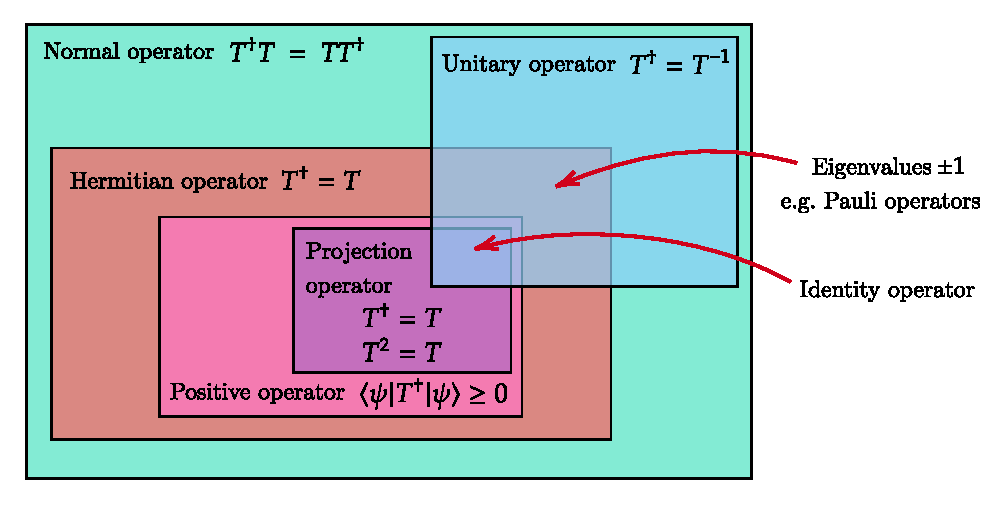
\includegraphics[scale=1]{fig/operator-classification.pdf}
	\caption{Taxonomy of linear operators that possess the spectral decomposition.}
	\label{fig:taxonomy}
\end{figure}

\begin{lemma}\label{}
	Over the field $\C$, positivity implies Hermiticity.\mn{A counterexample over $\R$:
	\begin{align*}
	\mqty(x&y) &\mqty(2&2\\0&0) \mqty(x\\ y) \\ &= x^2 + y^2 + (x+y)^2 \ge 0	
	\end{align*}}
	\begin{align}
		\expval{\op T}{\psi}, \forall\ket{\psi}\in\hilb \implies \op T\dgg = \op T.
	\end{align}
\end{lemma}
\begin{proof}
 	Let $\op T$ be a positive operator. Write $\hat T = \op H + i\op G$, and let $\ket{g_j}$ be normalized eigenvectors of $\op C$ corresponding to eigenvalues $\lambda_j$. For
 	\begin{align}
 		0 \le \expval{\op T}{g_j} = \underbrace{\expval{\op H}{g_j}}_{\textrm{Real}} + i\lambda_j 
 	\end{align}
 	to be true, $\lambda_j$ must vanish for all $j$. Since $\op G$ is Hermitian and all its eigenvalues vanish, it must be the zero operator. Therefore, $ \op T$ is Hermitian.
\end{proof}

\begin{lemma}\label{}
	For any linear operator $\op T$, $\op T\dgg\op T$ and $\op T\op T\dgg$ are positive operators
\end{lemma}
\begin{proof}
	\begin{align}
		\expval{\op T\dgg \op T}{\psi} = (\bra{\psi} \op T\dgg)(\op T\ket{\psi}) = \norm{\op T\ket{\psi}}^2 \ge 0.
	\end{align}
\end{proof}

\begin{lemma}\label{}
    $\op T\dgg \op T = \op\id \iff \op T\op T\dgg = \op\id$ in finite dimensions.
\end{lemma}

\begin{proof}
    Suppose that $\{\ket{e_j}\}$ is an ONB. Since $\op T\dgg\op T=\op\id$, $\ket{f_j} = \op T\ket{e_j}$ also form an ONB. Furthermore,
    \begin{align}
        \ket{f_j} = \op T\ket{e_j} = \op T \op T\dgg \op T\ket{e_j} = \op T\op T\dgg \ket{f_j}.
    \end{align}
    
    to be true for any $j$, it must be the case that $\op T \op T\dgg=\op\id$. The proof in the inverse direction proceeds similarly.

    The proof fails in infinite dimension. Despite the fact that $\{\ket{f_j}\}$ is an orthonormal set of infinite cardinality, there is no guarantee that it spans $\hilb$. For an explicit counterexample, consider the left shift $\op L$ \eqref{eq:left-shift} and the right shift $\op R$ \eqref{eq:right-shift}. They are adjoints of each other (check this!), and it is evident that $\op L\op R =\op\id$, but $\op R\op L\neq \op\id$ because the left shift irrecoverbly kills the first component of any vector.
\end{proof}



